\exercice On considère le quadrilatère tournant vu lors d'une activité:\\[1em] \noindent
$ABCD$ représente une feuille au format~$A4$ c'est-à-dire un rectangle de côtés $AB = 29,7cm$ et $BC = 21cm$.\\
On place $M$ sur $[AB]$.\\
On place ensuite $N$ sur $[BC]$, $P$ sur $[CD]$ et $Q$ sur $[DA]$ tels que~:\\ $AM = BN = CP = DQ$\\[1em]
On pose $x$ la longueur $AM$.
\begin{center}
	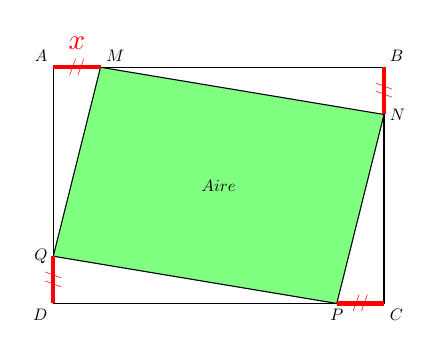
\begin{tikzpicture}[scale=0.6,every node/.style={scale=0.6}]
	\coordinate (A) at (0,0);
	\coordinate (B) at (7,0);
	\coordinate (C) at (7,-5);
	\coordinate (D) at (0,-5);
	\coordinate (M) at (1,0);
	\coordinate (N) at (7,-1);
	\coordinate (P) at (6,-5);
	\coordinate (Q) at (0,-4);
	\coordinate (S) at (7/2,-5/2);
	\draw (A) rectangle ++(7,-5);
	\draw (A)--(B)--(C)--(D)--cycle;
%	\draw [very thick,red] (A)--(M) node [midway,above] {$x$};
	\draw [black,fill=green!50] (M)--(N)--(P)--(Q)--cycle;
	\draw (A) node[above left] {$A$};
	\draw (B) node[above right] {$B$};
	\draw (C) node[below right] {$C$};
	\draw (D) node[below left] {$D$};
	\draw (M) node[above right] {$M$};
	\draw (N) node[right] {$N$};
	\draw (P) node[below] {$P$};
	\draw (Q) node[left] {$Q$};
	\draw (S) node {$Aire$};
%	\foreach \point in {A, B, C, D}
%		\draw (\point) node[above left] {$\point$};
	\draw [red,ultra thick] (A)--(M)node[midway,sloped]{$//$};
	\draw [red,ultra thick] (B)--(N)node[midway,sloped]{$//$};
	\draw [red,ultra thick] (C)--(P)node[midway,sloped]{$//$};
	\draw [red,ultra thick] (D)--(Q)node[midway,sloped]{$//$};
	\draw (0.5,0.5) node [scale=1.75,red] {$x$};
\end{tikzpicture}

\end{center}

\begin{enumerate}
	\item Montrez que les triangles $AMQ$ et $CPN$ sont identiques.
	\item De même pour les triangles $BNM$ et $DQP$.
	\item Déterminez l'aire totale de la surface recouverte par les 4 triangles précédents.
	\item Faites une phrase qui décrit le fait que l'aire verte peut s'écrire comme une fonction de $x$ dont on précisera le domaine de définition.
	\item Montrez que cette fonction a pour expression : \[a(x) = 2x^2 - 50,7x + 623,7\]
	\item Déterminez le minimum de cette fonction par le moyen de votre choix : lecture graphique, approximation par différents essais\ldots
\end{enumerate}